\chapter{Architecture and use cases}

\section{Generating GPU accelerated libraries}
In this thesis, we are interested in making Futhark-generated GPU kernels available
in \csharp{} programs.
Currently, Futhark source code can be compiled to C and Python code.
In example, the Futhark C compiler follows the basic architecture shown in
figure \ref{fig:ccompiler}.
When we call the Futhark C compiler \texttt{futhark-c} on a Futhark source file, the compiler reads
the source code file (and possibly imports) into the compiler.
The compiler optimizes the input program, and expresses it in a
compiler-internal intermediate language. This intermediate language code is then
passed to a code generator, which is expresses the intermediate language code in
C, and writes the result to a C source file.\\
This file can then be used in any other C program.

For Python compilation, exchange ``C'' for ``Python''.

\begin{figure}[H]
  \centering
  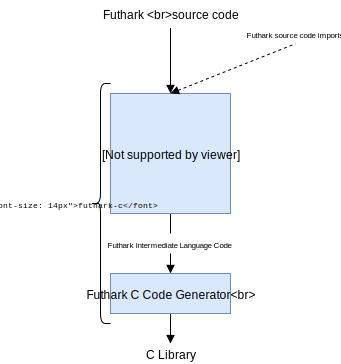
\includegraphics{chapters/figs/architecture/ccompiler.pdf}
  \caption{The Futhark-to-C compilation pipeline}
  \label{fig:ccompiler}
\end{figure}

\subsection*{Using Futhark in Python}
We will now describe a use case for the Futhark-to-Python compiler:
\begin{enumerate}
\item We write a short Futhark program, which has a single entry function
  available. This program takes an array of integers, and
adds 2 to each element in the array. The program is shown in figure \ref{fig:shortfutharkprogram0}. 
\item We then compile the Futhark program into a library file, by calling the
  Futhark compiler from the command line, like shown in figure \ref{fig:shortfutharkprogram1}.
This compiles \texttt{mapPlus2.fut} to a Python file called MapPlus2.py

\item Finally, we write a short Python program in which we want to integrate
  the mapPlus2 function in our program. Such a program is shown in figure \ref{fig:shortfutharkprogram2}.
  In this program, we are importing the Futhark library on line 1 and constructing
  an instance of the contained Futhark class on line 5.\\
  On line 4, we generate an array of integers from 0 to 1000000, and finally
  on line 6, we use the exposed Futhark function mapPlus2 to add 2 to every
  element in our array.
\end{enumerate}

\begin{figure}
\begin{lstlisting}[language=Futhark]
entry mapPlus2 (xs : []i32) : []i32 =
map (+2) xs
\end{lstlisting}
\caption{A short Futhark program called mapPlus2.fut}
\label{fig:shortfutharkprogram0}
\end{figure}

  \begin{figure}
\begin{lstlisting}[language=bash]
  $ futhark-py --library -o MapPlus2.py mapPlus2.fut
    \end{lstlisting}
    \caption{We call the Futhark-to-Python compiler \texttt{futhark-py} on
      mapPlus2.fut}
    \label{fig:shortfutharkprogram1}
  \end{figure}
  
  \begin{figure}
\begin{minted}[linenos]{python}
  from MapPlus2 import MapPlus2

  def main():
    xs = range(1,1000000)
    mapPlus2Class = MapPlus2()
    xs2 = mapPlus2Class.mapPlus2(xs)
  \end{minted}
    \caption{We use the compiled Futhark program as any other library.}
    \label{fig:shortfutharkprogram2}
  \end{figure}
\clearpage

\subsection*{How a Futhark-to-\csharp{} would be used}
We will now describe a use case for the Futhark-to-\csharp{} compiler:
\begin{enumerate}
\item We write a short Futhark program, which has a single entry function
  available. This program takes an array of integers, and
adds 2 to each element in the array. The program is shown in figure \ref{fig:shortfutharkprogram3}. 
\item We then compile the Futhark program into a library file, by calling the
  Futhark compiler from the command line, like shown in figure \ref{fig:shortfutharkprogram4}.
This compiles \texttt{mapPlus2.fut} to a \csharp{} file called MapPlus2.cs

\item Finally, we write a short \csharp{} program in which we want to integrate
  the mapPlus2 function in our program. Such a program is shown in figure \ref{fig:shortfutharkprogram5}.
  In this program, we are importing the Futhark library on line 2 and constructing
  an instance of the contained Futhark class on line 8.\\
  On line 9, we generate an array of integers from 0 to 1000000, and finally
  on line 10, we use the exposed Futhark function mapPlus2 to add 2 to every
  element in our array.
\end{enumerate}
\begin{figure}[H]
  \centering
  \begin{lstlisting}[language=Futhark]
entry mapPlus2 (xs : []i32) : []i32 =
  map (+2) xs
  \end{lstlisting}
  \caption{A short Futhark program called mapPlus2.fut}
  \label{fig:shortfutharkprogram3}
\end{figure}

\begin{figure}[H]
  \centering
  \begin{lstlisting}[language=sh]
$ futhark-cs --library -o MapPlus2.cs mapPlus2.fut
  \end{lstlisting}
  \caption{We call the Futhark-to-\csharp{} compiler \texttt{futhark-cs} on
    mapPlus2.fut}
  \label{fig:shortfutharkprogram4}
\end{figure}

\begin{figure}[H]
  \centering
\begin{minted}[linenos]{csharp}
using System.Linq;
using MapPlus2;

public class Program
{
    public static int Main(string[] args)
    {
        var mapplus2Class = new MapPlus2();
        var xs = Enumerable.Range(0, 1000000).ToArray();
        var xs_result = mapplus2Class.mapPlus2(xs)
    }
}
\end{minted}
  \caption{We use the compiled Futhark program as any other library.}
  \label{fig:shortfutharkprogram5}
\end{figure}

But to be able to achieve this, we must design and implement a Futhark \csharp{}
code generator.

\section{Obtaining and integrating GPU kernels from- and in high level
  languages}
Our second goal of this thesis is to create an architecture which lets us obtain
GPU kernels from high level language code, and afterwards integrate these
kernels back into the high level language program.
Specifically, we want to obtain GPU kernels from \fsharp{} source code, and
use these kernels in \fsharp{} programs afterwards.

In figure \ref{}, we show such an architecture for the \fsharp{} language.

\subsection{A use case}
\begin{enumerate}
\item  source code
\item  send for translation
\item  use function immediately
\end{enumerate}

\begin{figure}[h]
  \centering
\begin{minted}[linenos]{fsharp}
let saxpy (a : int) (x : int) (y : int) : int =
  a*x+y
  
[<FSharkEntry>]
let run_saxpy (a : int) (xs : int array) (ys : int array): int array =
  let res = Map2 (saxpy a) xs ys
  in res
\end{minted}
\caption{A short \fshark{} module called MapPlus2.fs}
\label{fig:shortfsharkprogram0}
\end{figure}


\begin{figure}[h]
  \centering
\begin{minted}[linenos]{fsharp}
[<EntryPoint>]
let main =
  let fshark = new FShark()
  fshark.addSourceFile("MapPlus2.fs")
  fshark.CompileAndLoad()

  let a = 5
  let xs = Iota 10000
  let ys = Replicate 10000 1
  let res = fshark.InvokeFunction("run_saxpy", a, xs, ys)
\end{minted}
  \caption{Compiling and using MapPlus2.fs from within an \fsharp{} program.}
  \label{fig:shortfsharkprogram1}
\end{figure}



%%% Local Variables:
%%% mode: latex
%%% TeX-master: "../thesis"
%%% End:
